\chapter{Arduino}\label{analysis:arduino}
Arduino was created in Italy at the Interaction Design Institute Ivrea, by Massimo Banzi and David Cuartielles. They where looking for an easy and cheap way for design-students, to integrate micro controllers in the projects\cite{arduino:hist}. Both the board and the programming language was based on the works of Hernando Barragán, one of Massimo Banzi master thesis students \cite{Wiring:thesis}

\section{The hardware components}
Arduino is a single-board micro-controller, see the pictures in figure \ref{fig:Arduino}.
A board consists of open source hardware, which is designed around an 8-bit Atmel AVR micro-controller. Arduino boards varies in sizes. Arduino Uno board for example, has a max width of 2.1'' (5,33cm) and a length of 2.7'' (6,86cm).  \\

\par
\raisebox{-.5\height}{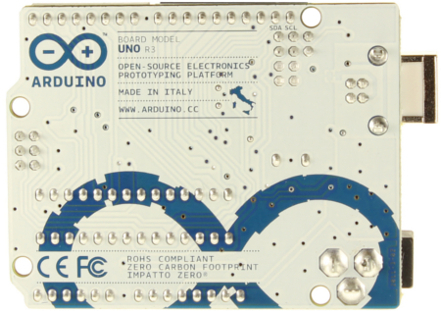
\includegraphics[width=6.5cm]{billeder/ArduinoUno_R3_Back_450px.jpg}}
\hfill
\raisebox{-.5\height}{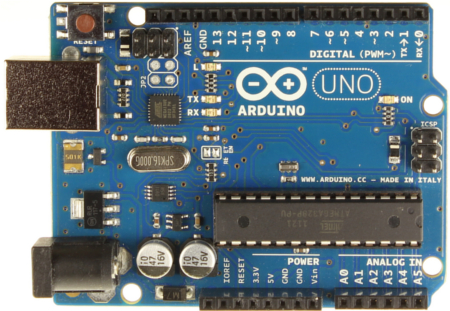
\includegraphics[width=6.5cm]{billeder/ArduinoUno_R3_Front_450px.jpg}}
\begin{figure}[H]
\caption{Picture of back- and fronside of the Arduino board}
\label{fig:Arduino}
\end{figure}
\par

The board provides some input and output possibilities. However these varies depending on the board, though most have 14 digital I/O and 6 analog inputs. The I/O functions are placed on top of the board, are freely accessible, and consist of 0.1'' female headers. Besides the I/O there is also a Power connector, which almost in all cases require 5 volt DC. There is an USB connection on the board, so that processing data to the micro-controller is possible, though it is shown as a virtual com-port on the connected computer. However, on older boards, instead of the USB connection, a RS232 were used for serial communication. 

On the board there is an LED diode which is connected to the digital pin 13. When this diode is set to ``HIGH'' it will be turned on, and if its value is ``LOW'' it turns off. Besides the LED diode, there is also a reset button. If the button is pressed the micro-controller is reset. 

Arduino board gain extra features through shields. Shields is a ``board'', or rather an expansion board, which is plugged onto the Arduino board. This provides Arduino boards with the possibilities to control extra components for example motors, sensors and LCD displays.

\section{The Arduino language}
The Arduino language is based on Wiring and therefore there are a lot of similarities between the two languages, but the Arduino team have added to, improved the functions, and made it compatible with a wider range of chips. Also, both languages are implemented as a  version of C/C++, and are using an IDE based on the processing IDE \cite{Wiring:thesis}\cite{Arduino:IDE}.\\

\begin{table}[H]
\centering
\begin{tabular}{cc}
Wiring 
& 
Arduino \\ 
\hline 
\begin{lstlisting}
int ledPin = 8;

void setup(){
  pinMode(ledPin, OUTPUT);
}
void loop(){
  digitalWrite(ledPin, HIGH);
  delay(1000);
  digitalWrite(ledPin, LOW);
  delay(1000);
}
\end{lstlisting}  
& 
\begin{lstlisting}
int led = 13;

void setup() {                
  pinMode(led, OUTPUT);     
}
void loop() {
  digitalWrite(led, HIGH);
  delay(1000);
  digitalWrite(led, LOW);
  delay(1000);
}
\end{lstlisting} 
\end{tabular} 
\caption{Blink examples take from the Wiring and Arduino resources}
\label{tabel:comparison}
\end{table}

As can be seen from table \ref{tabel:comparison}, the syntax of the two languages are almost identical, and it is only in the functions parameters, that there are any noticeable difference.\\ 
To help facilitate the compatibility with a wide range of AVR chips, the Arduino language makes great use of AVR Libc \cite{AVR:lib}, which is an open source C library that supplies the necessary functionality to make it possible to use the Atmel AVR micro controllers.